\chapter{Anforderungsdefinition und Modellierung}
\label{cha:Anforderungsdefinition und Modellierung}


\section{Anforderungen}
\label{sec:Anforderungen}
Im nachfolgenden Abschnitt definieren wir die funktionalen Anforderungen der Software. Wir bestimmten, welche Funktionalitäten die Strategiespiele und die Agenten mindestens haben und wie die Agenten getestet werden sollen. Wir definieren die Funktionalitäten, um den Funktionsbereich der Software einzugrenzen und einen Überblick zu verschaffen.

\subsection{Tic Tac Toe Spielumgebung}
Die Spielumgebung soll die in Abschnitt \ref{sec:Das Strategiespiel Tic Tac Toe} definierten Tic Tac Toe Spielregeln implementieren. Die Tic Tac Toe Spielumgebung repräsentiert eine Testumgebung für die Agenten, der Zufallsagent wird in dieser Umgebung gegen den TicTacToe-Heuristik Agenten antreten. Der TD-Q-Lernende Agent soll zuerst diese Umgebung erkunden und lernen sich in der Umgebung zurecht zu finden, d.h. der TD-Q-Lernende Agent soll eine TicTacToe-Siegesstrategie entwickeln. 

\myparagraph{makeMove(position):}
Die Funktion soll Koordinaten erhalten. Die Koordinaten definiert exakt, auf welches Spielfeld eine Spielfigur gesetzt werden soll. Die Funktion soll diesen Spielzug, sollte dieser Regelkonform sein, ausführen.

\myparagraph{undoMove():}
Die Funktion soll den letzten durchgeführten Spielzug revidieren.

\myparagraph{getPossibleMoves(): return list}
Die Funktion soll eine Liste von Koordinaten liefern. In dieser Liste sind nur mögliche und regelkonforme Spielzüge (Koordinaten) enthalten.

\myparagraph{getPlayerToMove(): return str}
Die Funktion soll String zurückgeben, dieser String repräsentiert den Spieler der aktuell einen Spielzug ausführen soll. Der String ''X'' ist die Repräsentation des Kreuzspielers. Der String ''O'' ist die äquivalente Repräsentation des Kreisspielers.

\myparagraph{isTerminal: return bool}
Die Funktion soll True zurück liefern, wenn der aktuelle Zustand der Umgebung ein Endzustand (Terminalzustand) ist, andernfalls liefert die Funktion ein False.

\myparagraph{getReward: return float}
Die Funktion soll eine nummerische Belohnung liefern. Die Belohnung soll abhängig sein vom aktuellen Spielzustand.

\subsection{Reversi Spielumgebung}
Die Spielumgebung soll die in Abschnitt \ref{sec:Das Strategiespiel Reversi} definierten Reversi Spielregeln implementieren. Die Reversi Spielumgebung repräsentiert eine Testumgebung für die Agenten, der Zufallsagent wird in dieser Umgebung gegen den Reversi-Heuristik Agenten antreten. Der TD-Q-Lernende Agent soll zuerst diese Umgebung erkunden und lernen sich in der Umgebung zurecht zu finden, d.h. der TD-Q-Lernende Agent soll eine Reversi-Siegesstrategie entwickeln. 

\myparagraph{makeMove(position):}
Die Funktion soll Koordinaten erhalten. Die Koordinaten definiert exakt, auf welches Spielfeld eine Spielfigur gesetzt werden soll. Die Funktion soll diesen Spielzug, sollte dieser Regelkonform sein, ausführen.

\myparagraph{undoMove():}
Die Funktion soll den letzten durchgeführten Spielzug revidieren.

\myparagraph{getPossibleMoves(): return list}
Die Funktion soll eine Liste von Koordinaten liefern. In dieser Liste sind nur mögliche und regelkonforme Spielzüge (Koordinaten) enthalten.

\myparagraph{getPlayerToMove(): return str}
Die Funktion soll String zurückgeben, dieser String repräsentiert den Spieler der aktuell einen Spielzug ausführen soll. Der String ''B'' ist die Repräsentation des schwarzen (black) Spielers. Der String ''W'' ist die äquivalente Repräsentation des weißen (white) Spielers.

\myparagraph{isTerminal: return bool}
Die Funktion soll True zurück liefern, wenn der aktuelle Zustand der Umgebung ein Endzustand (Terminalzustand) ist, andernfalls liefert die Funktion ein False.

\myparagraph{getReward: return float}
Die Funktion soll eine nummerische Belohnung liefern. Die Belohnung soll abhängig sein vom aktuellen Spielzustand.

\subsection{Agent des Zufalls}
Der Agent des Zufalls soll den schlechtesten Spieler symbolisieren. Er soll seine Entscheidungen vollkommen zufällig treffen. In Kapitel \ref{cha:Validierung} Validierung werden wir diesen Agenten, als Gegenspieler für die Heuristik Agenten und die lernenden TD-Q-Agenten einsetzen. \\

\myparagraph{suggestRandomTicTacToeAction(ticTacToeState): return tuple}
Diese Funktion soll eine Tic Tac Toe Spielsituation übergeben bekommen, d.h. eine Instanz der TicTacToe Klasse. Die Funktion soll eine zufällige, aber zulässige, Aktion zurückgeben.

\myparagraph{suggestRandomReversiAction(reversiState): return tuple}
Diese Funktion soll eine Reversi Spielsituation übergeben bekommen, d.h. eine Instanz der Reversi Klasse. Die Funktion soll eine zufällige, aber zulässige, Aktion zurückgeben.

\subsection{Tic Tac Toe Heuristik Agent}
Der Agent soll die in Abschnitt \ref{subsec:Heuristik} erstellte Tic Tac Toe Heuristik und eine 2-Spielzüge vorausschauende Alpha-Beta Suche verwenden (siehe Abschnitt \ref{subsec:Iterativ vertiefende Tiefensuche} und \ref{subsec:Alpha-Beta-Kürzung}). Dieser Agent soll einen fortgeschrittenen Spielgegner repräsentiert, d.h. wir müssen mittels Testspielen gegen den Zufallsagenten zeigen, dass der Tic Tac Toe Heuristik Agent verhältnismäßig oft gewinnt. Dieser Agent soll in Tic Tac Toe Testspielen gegen den TD-Q-Agenten antreten. Die Ergebnisse sollen dabei helfen, die Leistungsfähigkeit und Grenzen des TD-Q-Lernens, hinsichtlich dem Lernen von Tic Tac Toe, zu beurteilen. 

\myparagraph{suggestAction(ticTacToeState): return tuple}
Diese Funktion soll eine Tic Tac Toe Spielsituation übergeben bekommen. Die Funktion soll, abhängig von der erhaltenen Spielsituation, eine Aktion vorschlagen. Die Aktion soll mittels der TicTacToe-Heuristik und eienr 2-Zug Vorausschau und Alpha-Beta-Suche ermittelt werden.

\subsection{Reversi Heuristik Agent}
Der Agent soll die in Abschnitt \ref{subsec:Heuristik} erstellte Reversi Heuristik und eine 2-Spielzüge vorausschauende Alpha-Beta Suche verwenden (siehe Abschnitt \ref{subsec:Iterativ vertiefende Tiefensuche} und \ref{subsec:Alpha-Beta-Kürzung}). Dieser Agent soll einen fortgeschrittenen Spielgegner repräsentiert, d.h. wir müssen mittels Testspielen gegen den Zufallsagenten zeigen, dass der Reversi-Heuristik Agent verhältnismäßig oft gewinnt. Dieser Agent soll in Reversi Testspielen gegen den TD-Q-Agenten antreten. Die Ergebnisse sollen dabei helfen, die Leistungsfähigkeit und Grenzen des TD-Q-Lernens, hinsichtlich dem Lernen von Reversi, zu beurteilen.

\myparagraph{suggestAction(reversiState): return tuple}
Diese Funktion soll eine Reversi Spielsituation übergeben bekommen. Die Funktion soll, abhängig von der erhaltenen Spielsituation, eine Aktion vorschlagen. Die Aktion soll mittels der Reversi Heuristik und eienr 2-Zug Vorausschau und Alpha-Beta-Suche ermittelt werden.

\subsection{Tic Tac Toe TD-Q lernender Agent}
Der Agent soll, mittels des in Abschnitt \ref{sec:TD-Q-Lernen} behandelten TD-Q-Lernens, eine Siegesstrategie für das Strategiespiel Tic Tac Toe entwickeln. Testspiele gegen den Zufallsagenten und den Tic Tac Toe Heuristik Agenten, sollen eine Untersuchung der Leistungsfähigkeit und der Grenzen des TD-Q-Lernens ermöglichen.

\myparagraph{learnTicTacToeInXGames(amountOfGames):}
Die Funktion soll den Lernmodus des Agenten realisieren. Der Eingabeparameter legt die Anzahl der Trainingsspiele fest. Die Lernerfahrungen während dieser Trainingsspiele, sollen in einer SQLite Datenbank gespeichert werden.

\myparagraph{suggestAction(ticTacToeState): return tuple}
Die Funktion soll eine Tic Tac Toe Spielsituation übergeben bekommen. Ausgehend von der Eingangsspielsituation, ist nur eine bestimmte Anzahl von Aktionen möglich. Abhängig von seinen Erfahrungen und dem gegebenen Spielzustand, soll der Agent die mögliche Aktion mit dem höchsten gelernten Q-Wert zurückgeben.

\subsection{Reversi TD-Q lernender Agent}
Der Agent soll, mittels des in Abschnitt \ref{sec:TD-Q-Lernen} behandelten TD-Q-Lernens, eine Siegesstrategie für das Strategiespiel Reversi entwickeln. Testspiele gegen den Zufallsagenten und den Reversi Heuristik Agenten, sollen eine Untersuchung der Leistungsfähigkeit und der Grenzen des TD-Q-Lernens ermöglichen.

\myparagraph{learnReversiInXGames(amountOfGames):}
Die Funktion soll den Lernmodus des Agenten realisieren. Der Eingabeparameter legt die Anzahl der Trainingsspiele fest. Die Lernerfahrungen während dieser Trainingsspiele, sollen in einer SQLite Datenbank gespeichert werden.

\myparagraph{suggestAction(reversiState): return tuple}
Die Funktion soll eine Reversi Spielsituation übergeben bekommen. Ausgehend von der Eingangsspielsituation, ist nur eine bestimmte Anzahl von Aktionen möglich. Abhängig von seinen Erfahrungen und dem gegebenen Spielzustand, soll der Agent die mögliche Aktion mit dem höchsten gelernten Q-Wert zurückgeben.

\subsection{Testen der Agenten}
Eine Testumgebung, in der alle Agenten gegeneinander Spielen. Der Zufallsagent soll in 100 Testspielen gegen den Tic Tac Toe Heuristik Agenten, den Reversi Heuristik Agenten, den Tic Tac Toe TD-Q-Lernen Agenten und den Reversi TD-Q-Lernen Agenten antreten. Der Tic Tac Toe Heuristik Agent soll 100 Testspiele gegen die drei Lernstadien des Tic Tac Toe TD-Q-Lernen Agenten spielen. Im ersten Lernstadium soll der TD-Q-Lernen Agent, in 100 Trainingsspielen gegen sich selbst, eine Strategie entwickeln. Im zweiten Lernstadium sollen es 1000 und im dritten Lernstadium 10000 Trainingsspiele sein. Äquivalent gilt dies auch für den Reversi TD-Q-Lernen Agenten und den Reversi Heuristik Agenten. Selbstverständlich spielen die Reversi Agenten, in der Reversi Spielumgebung und die Tic Tac Toe Agenten, in der Tic Tac Toe Spielumgebung.
\newpage

\section{Modellierung}

\begin{figure}[!htbp]
  \centering
  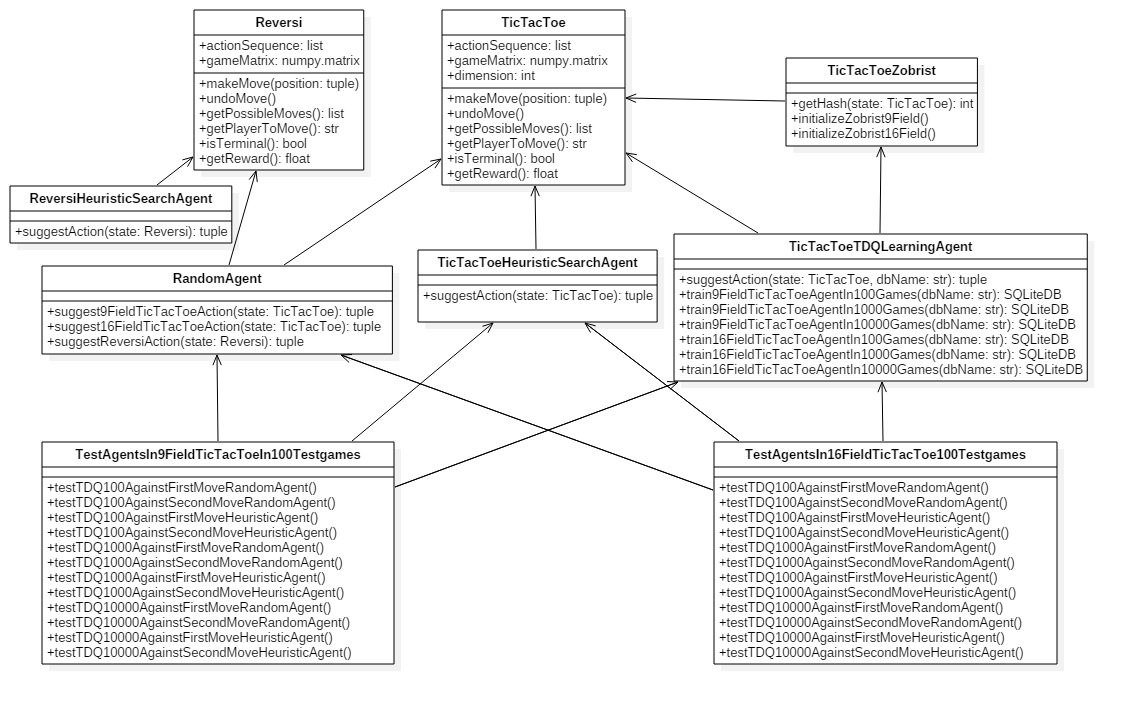
\includegraphics[angle = 90, scale = 0.5]{inhalt/abbildungen/projectClassDiagram.jpg}
  \caption{Klassendiagramm der Software}
  \label{fig:klassendiagramm}
\end{figure} 
